\documentclass{beamer}
%Information to be included in the title page:
% \title{Sample title}
% \author{Anonymous}
% \institute{Overleaf}
\usepackage{booktabs}
\usepackage{graphicx}

\usetheme[]{default}
\begin{document}
\renewcommand{\d}{\: \mathrm{d} }
\newcommand{\e}{\mathrm{e}}


% \frame{\titlepage}
% \title[] {Introduction to Semiconductor Devices}
\title[] {Recitation Class 1}

\author[lzx]{Zexi Li}

\institute[email]{lzx12138@sjtu.edu.cn}

\date{2021.05.18}

\frame{\titlepage}

\AtBeginSection[]
{
  \begin{frame}
    \frametitle{Table of Contents}
    \tableofcontents[currentsection]
  \end{frame}
}

\begin{frame}
    \frametitle{Outline}
    \tableofcontents
\end{frame}

% * Chapter 1
\section{Chapter 1: Crystalline structure of solids}
    \begin{frame} \frametitle{Semiconductor Materials}
        %\scalebox{0.8}{
            \begin{table}[H]
                \resizebox*{\textwidth}{!}{ %
                % \hspace{-4em}
                    \begin{tabular}{ccc}
                        \toprule
                        Conductors & Semiconductors & Insulators \\
                        \midrule
                        $< 10^{-3} \Omega \cdot \text{cm}$ & $10^{-3} - 10^9 \Omega \cdot \text{cm}$ & $> 10^9 \Omega \cdot \text{cm}$ \\
                        Metals (Au, Al, Cu, Hg, $\dots$) & Si, Ge, GaAs, InP, $\dots$ & SiO$_2$, HfO$_2$, $\dots$ \\
                        Solids, liquids (Hg) & Solids & Solids, liquids gases \\
                        \bottomrule
                    \end{tabular}
                }
                \caption{Semiconductor}
                \label{tab:Semiconductor}
            \end{table}

        \par \textbf{Semiconductors} are the materials that have resistivities between $10^{-3} - 10^9 \Omega \cdot \text{cm}$ depending on light illumination, temperature, electric field, magnetic field and impurities.
    \end{frame}

    \begin{frame} \frametitle{Type of Solids}
        \begin{figure}[H]
            \centering
            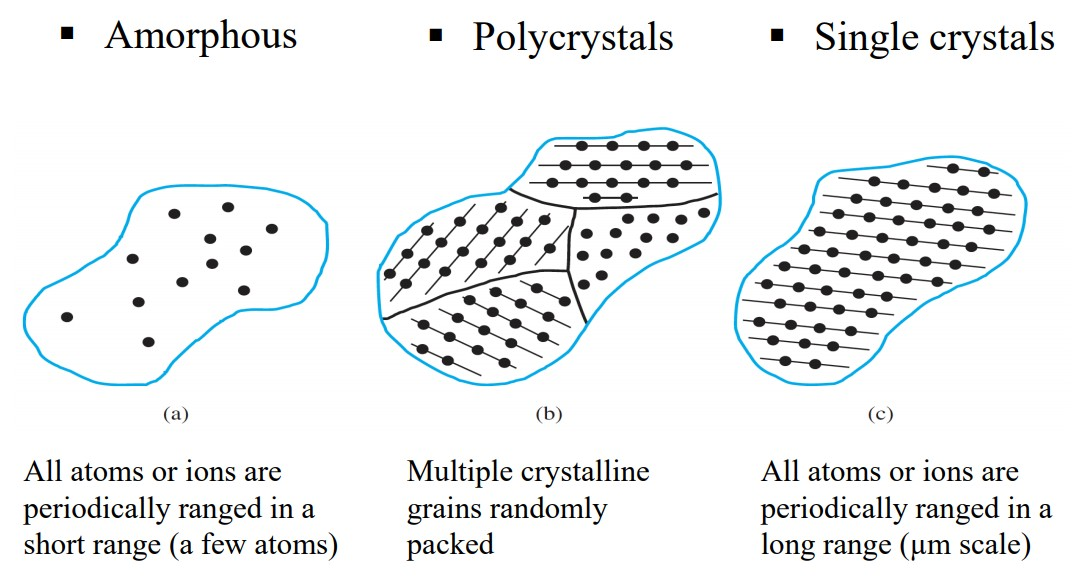
\includegraphics[width=0.95\linewidth]{Type_of_solids.jpg}
            \label{fig:Type_of_solids.jpg}
        \end{figure}
        \par All semiconductors covered in this course are assumed to be single crystalline.
    \end{frame}

    \begin{frame} \frametitle{Primitive and unit cell}
        \begin{figure}[H]
            \centering
            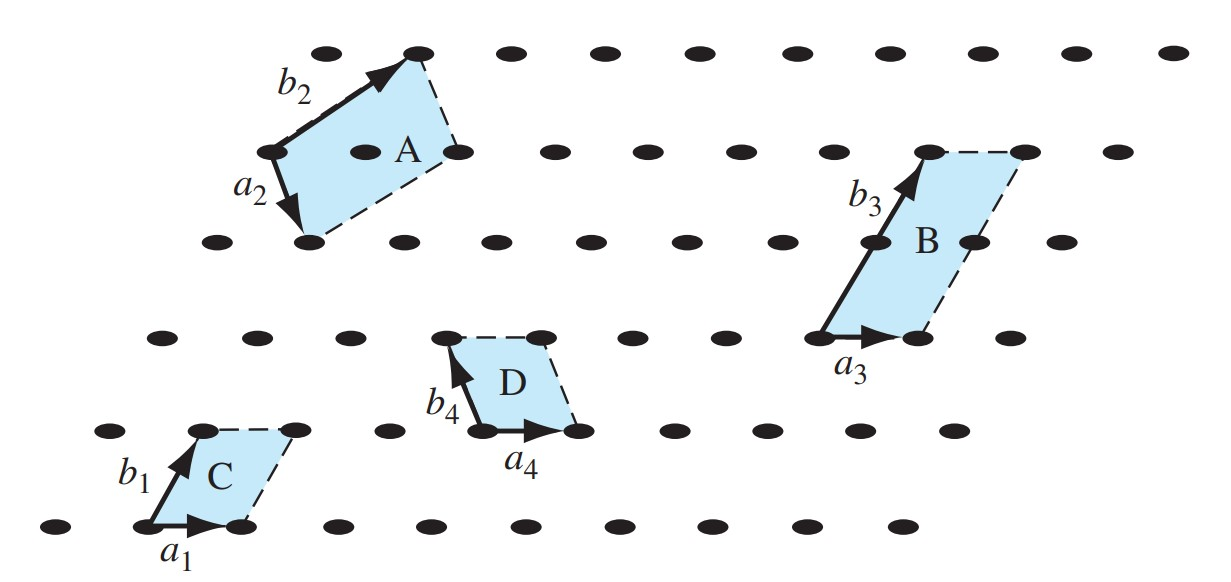
\includegraphics[width=0.6\linewidth]{Unit-cell.jpg}
            \label{fig:Unit-cell.jpg}
        \end{figure}
        \par \textbf{Unit Cell: } small volume of the crystal that can be used to reproduce the entire crystal. 
        \par A unit cell is not a unique entity
        \par \textbf{Primitive Cell: }  the smallest unit cell that can be repeated to form the lattice.
        
    \end{frame}

    \begin{frame} \frametitle{Lattice types}
        \begin{figure}[H]
            \centering
            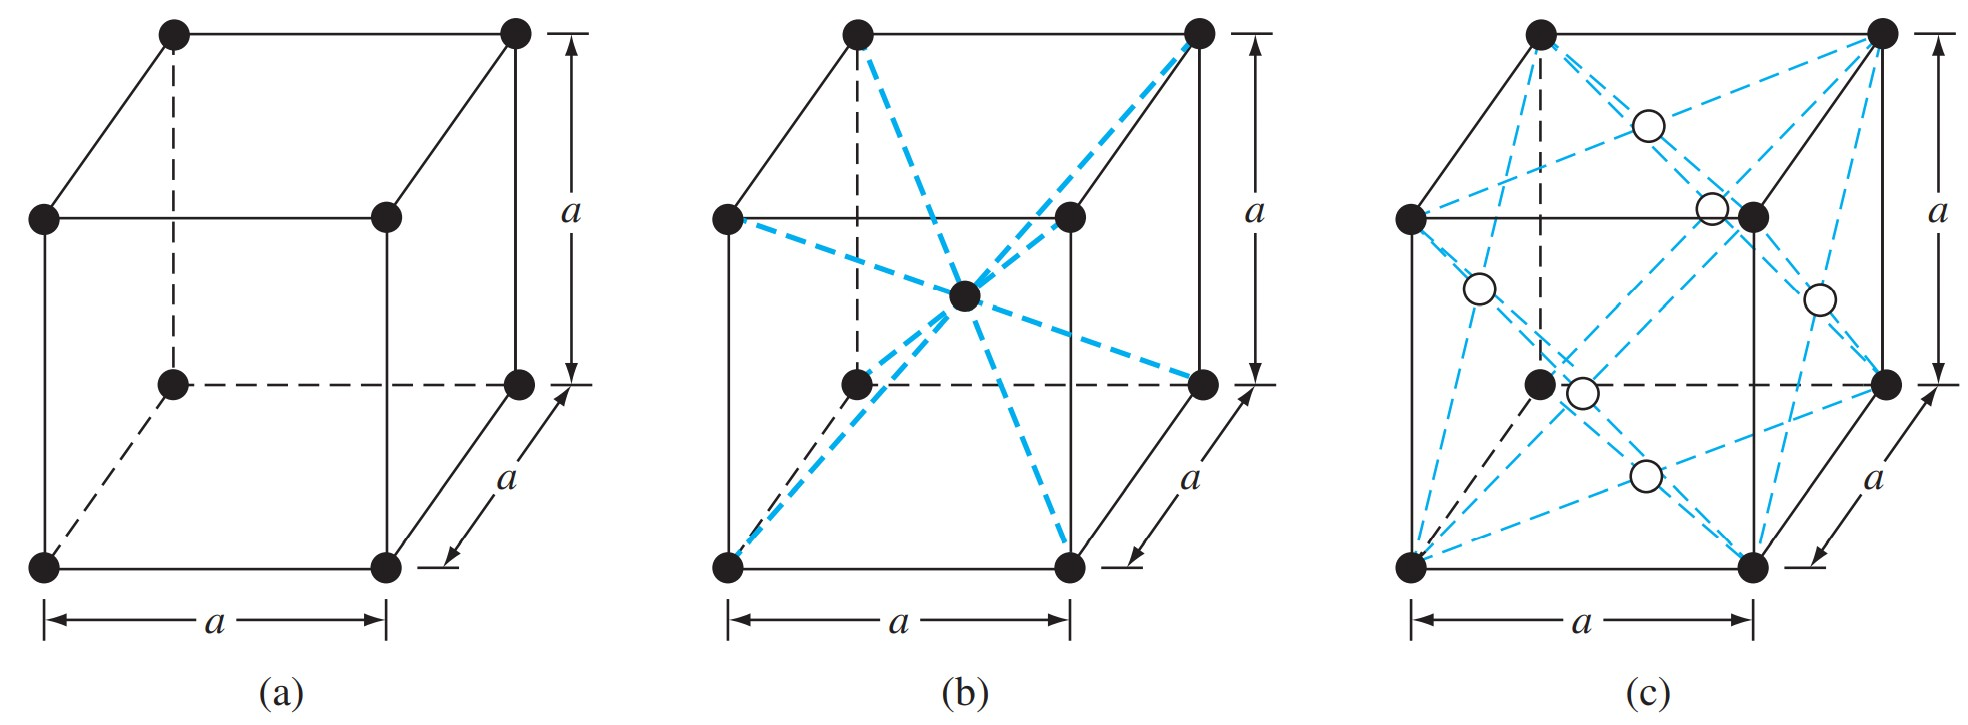
\includegraphics[width=0.9\linewidth]{Lattice_types.jpg}
            \caption{\tiny (a) simple cubic(\textcolor{red}{sc}), (b) body-centered cubic(\textcolor{red}{bcc}), (c) face-centered cubic(\textcolor{red}{fcc})}
            \label{fig:Lattice_types.jpg}
        \end{figure}
        \begin{equation*}
            \# \text{number of atoms per unit cell}
        \end{equation*}
        % volume density of atoms
        \begin{equation*}
            \text{Volume Density} = \frac{\text{\# atoms per unit cell}}{\text{volume of unit cell}} 
        \end{equation*}
        % Surface density of atoms
        \begin{equation*}
            \text{Surface Density} = \frac{\text{\# atoms per lattice plane}}{\text{area of lattice plane}}
        \end{equation*}
        (Example after reviewing Miller index)
    \end{frame}


    \begin{frame} \frametitle{The diamond structure}
        \par \textbf{The diamond structure } all atoms are of the same species
        \par \textbf{The zincblende structure } two different types of atoms. e.g, GaAs.
        % TODO: check this
        % No two atoms of same type are connected together.
        \begin{figure}[H]
            \centering
            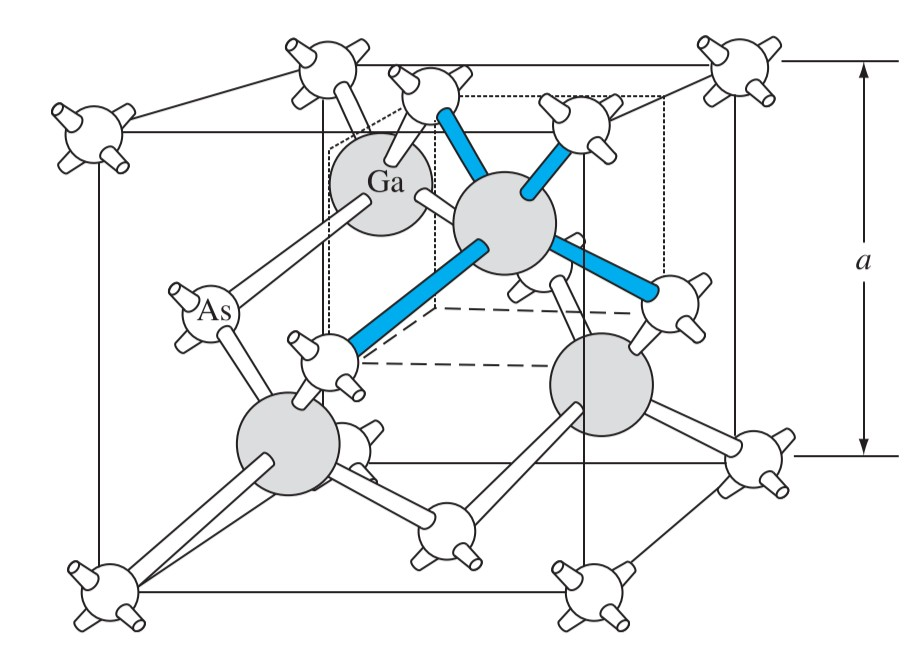
\includegraphics[width=0.5\linewidth]{GaAs_zincblende.jpg}
            \label{fig:GaAs_zincblende.jpg}
        \end{figure}
    \end{frame}

    \begin{frame} \frametitle{The diamond structure: To help remember}
        Method 1:
        \begin{figure}[H]
            \centering
            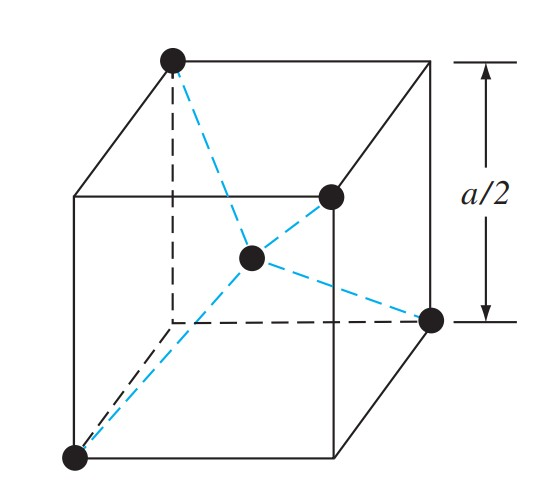
\includegraphics[width=0.2\linewidth]{Zincblend_tetrahedral_structure.jpg}
            \includegraphics[width=0.5\linewidth]{Zincblend_memory_method_1.jpg}
            \caption{Tetrahedral structure \& (a) bottom half, (b) top half}
            \label{fig:Zincblend_memory_method_1.jpg}
        \end{figure}

        Method 2:
        \begin{figure}[H]
            \centering
            \includegraphics[width=0.5\linewidth]{Zincblend_memory_method_2.jpg}
            \label{fig:Zincblend_memory_method_2.jpg}
        \end{figure}
        Equivalent to two face-centered cubics sliding $1/4$ diagonal length along a diagonal.
    \end{frame}

    \begin{frame} \frametitle{Crystalline Plane and Miller Index}
        \begin{figure}[H]
            \centering
            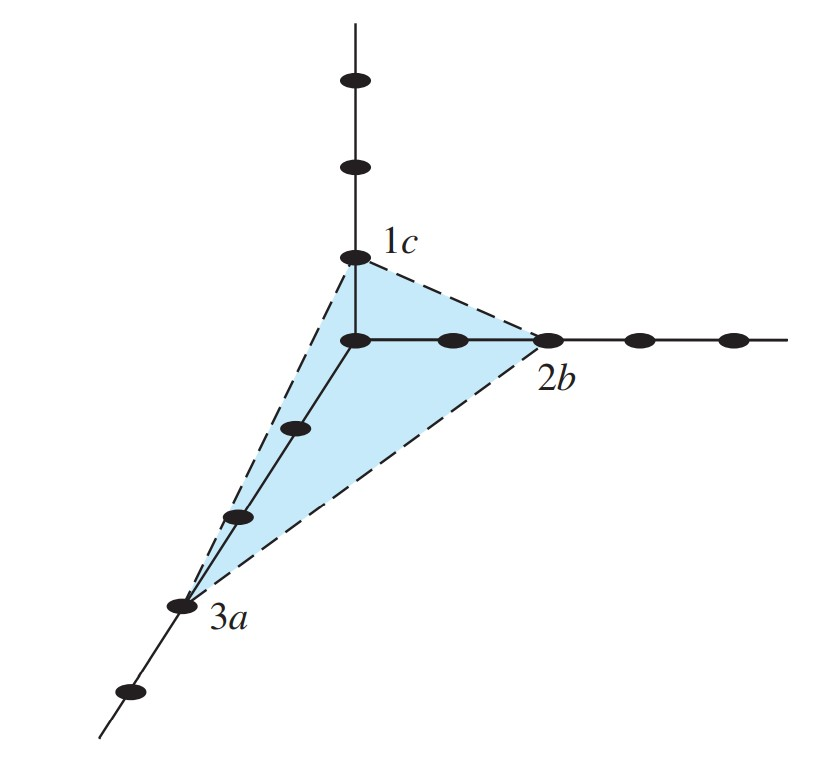
\includegraphics[width=0.4\linewidth]{Miller-index-1.jpg}
            \label{fig:Miller-index-1.jpg}
        \end{figure}
        % \par Intercepts: $(3,2,1)$.
        % \par Reciprocal: $(\frac{1}{3}, \frac{1}{2} , 1 )$.
        % \par Multiplying the lowest common denominator (lcd): $(2,3,6)$.
        \begin{equation*}
            (3,2,1) \stackrel{\text{Reciprocal}}{\longrightarrow} (\frac{1}{3} , \frac{1}{2} , 1) \stackrel{\text{multiply lcd}}{\longrightarrow} (2,3,6)
        \end{equation*}
        

        \par Any parallel plane is entirely equivalent to any other.

        \par The $[hkl]$ \underline{direction} is perpendicular to the $(hkl)$ \underline{plane}.
    \end{frame}

    \begin{frame} \frametitle{Example: Surface density}
        \par The lattice constant of a single crystal is $4.50 \; \mathring{A}$. Calculate the surface density of atoms (\# per $cm^2$) on the plane $(111)$ for face-centered cubic lattice.
        \begin{figure}[H]
            \begin{flushleft}
                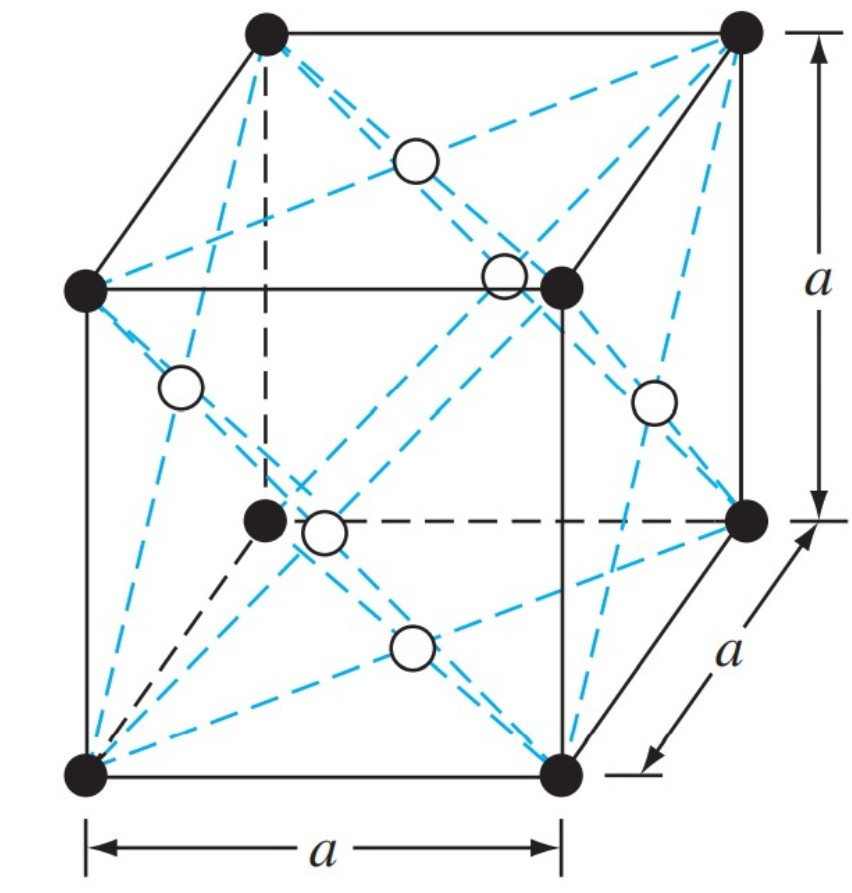
\includegraphics[width=0.4\linewidth]{Example-surface-density.jpg}
            \end{flushleft}
            \label{fig:Example-surface-density.jpg}
        \end{figure}
    \end{frame}

    \begin{frame} \frametitle{Doping}
        \par \textbf{n-type semiconductors:} Charge carriers are negative, i.e. electrons doped by donor-type of dopants.
        \par \textbf{p-type semiconductors:} Charge carriers are positive, i.e. holes doped by acceptor-type of dopants.
    \end{frame}


    % * Chapter 2
\section{Chapter 2: Quantum Mechanics}
    \begin{frame} \frametitle{Basic concepts}
        Wave function:
        \begin{equation*}
            \Psi(x)
        \end{equation*}
        Probability density function:
        \begin{equation*}
            \left| \Psi(x) \right|^2 = \Psi(x) \cdot \Psi^*(x)
        \end{equation*}
        Schrodinger Equation:
        \begin{equation*}
            - \frac{\hbar^2}{2m} \cdot \frac{\partial^2 \Psi(x, t)}{\partial x^2} + V(x) \Psi(x, t) = j \hbar \frac{\partial \Psi(x, t)}{\partial t}
        \end{equation*}
        \begin{equation*}
            \boxed{\frac{\partial^2 \psi(x)}{\partial x^2} + \frac{2m}{\hbar^2} \left( E - V(x) \right) \psi(x) = 0}
        \end{equation*}
        \begin{flushright}
            $E$: total energy of the particle.
        \end{flushright}
    \end{frame}
    \begin{frame} \frametitle{Infinite quantum well}
        \begin{equation*}
            - \frac{\hbar^2}{2m} \frac{\partial^2 \Psi}{\partial x^2} + V(x) \Psi = E \Psi  , \quad \left\{
                \begin{array}{ll}
                    V(x) = + \infty, & x \le 0 \text{ or } x \ge a \\
                    V(x) = 0, & 0 < x < a
                \end{array}
            \right.
        \end{equation*}
        General solution:
        \begin{equation*}
            \Psi (x) = A \e^{-ikx} + B \e^{ikx} 
        \end{equation*}
        Boundary condition:
        \begin{equation*}
            \begin{aligned}
            % \left\{
                % \begin{array}{ll}
                    & \Psi (x) | _{x = a, 0} = 0 \\
                    & \int_{0}^{a} \Psi(x) \Psi^*(x) \d x = 1 \\
                % \end{array}
            % \right.
            \end{aligned}
        \end{equation*}
        conclusion:
        \begin{equation*}
            \begin{aligned}
                &k = \frac{n\pi}{a} , n = 0, \pm 1, \pm 2, \dots \\
                &E = \frac{k^2 \hbar^2}{2m} = \frac{n^2 \pi^2 \hbar^2}{2m a^2}  
            \end{aligned}
        \end{equation*}
    \end{frame}


    \begin{frame} \frametitle{Finite quantum well}
        \begin{equation*}
            - \frac{\hbar^2}{2m} \frac{\partial^2 \Psi}{\partial x^2} + V(x) \Psi = E \Psi  , \quad \left\{
                \begin{array}{ll}
                    V(x) = V_0, & x \le 0 \text{ or } x \ge a \\
                    V(x) = 0, & 0 < x < a
                \end{array}
            \right.
        \end{equation*}
        General solution:
        \begin{equation*}
            \Psi(x) = 
            \left\{
                \begin{array}{lll}
                    A \e^{-i k_1 x} + B \e^{ik_1 x}, & k_1 = \sqrt{\frac{2m(E - V_0)}{\hbar^2} } , & x \le 0\text{ or }x \ge a \\
                    C \e^{-ik_2x} + D \e^{ik_2 x}, & k_2 = \sqrt{\frac{2mE}{\hbar^2} } , & 0 < x < a 
                \end{array}
            \right.
        \end{equation*}
        Boundary condition:
        \begin{equation*}
            \begin{aligned}
            % \left\{
                % \begin{array}{ll}
                    & \Psi (x) | _{x = 0} \text{ continuous}\\
                    & \Psi (x) | _{x = a} \text{ continuous}\\
                    & \int_{-\infty}^{\infty} \Psi(x) \Psi^*(x) \d x = 1 \\
                % \end{array}
            % \right.
            \end{aligned}
        \end{equation*}
        Note: depending on the relationship between $E$ and $V_0$, $\Psi(x)$ is different.
    \end{frame}

    \begin{frame} \frametitle{Example}
        Consider the one-dimensional potential function shown in the figure below. Assume the total energy of an electron is $E < V_0$.
        \begin{enumerate}[a)]
            \item Write the wave solutions that apply in each region.
            \item Write the set of equations that result from applying the boundary conditions.
            \item Show explicitly why, or why not, the energy levels of the electron are quantized.
        \end{enumerate}
        \begin{figure}[H]
            \centering
            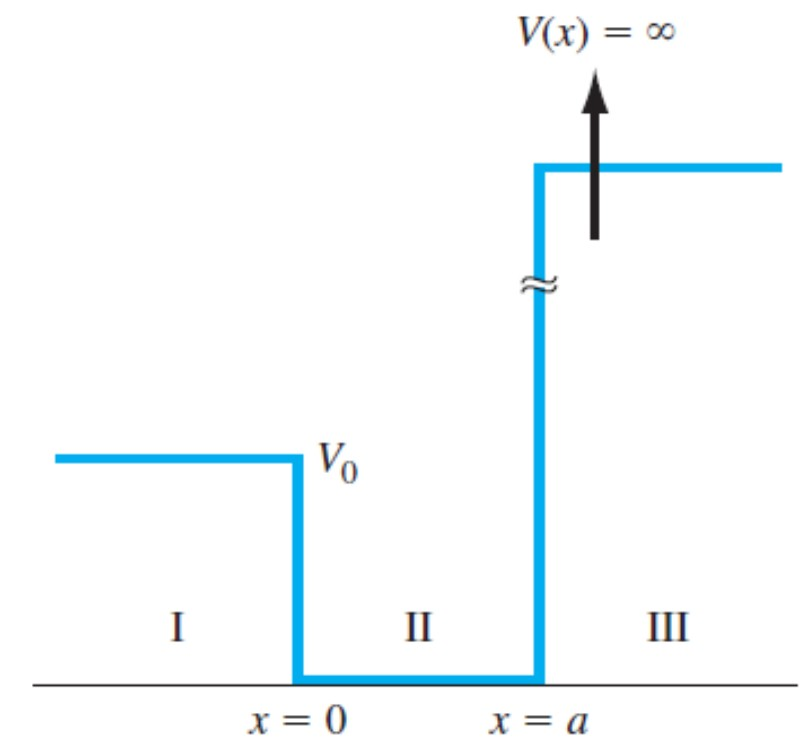
\includegraphics[width=0.4\linewidth]{Example-quantum-well.jpg}
            \label{fig:Example-quantum-well.jpg}
        \end{figure}
    \end{frame}

    \begin{frame} \frametitle{Example}
        \begin{figure}[H]
            \centering
            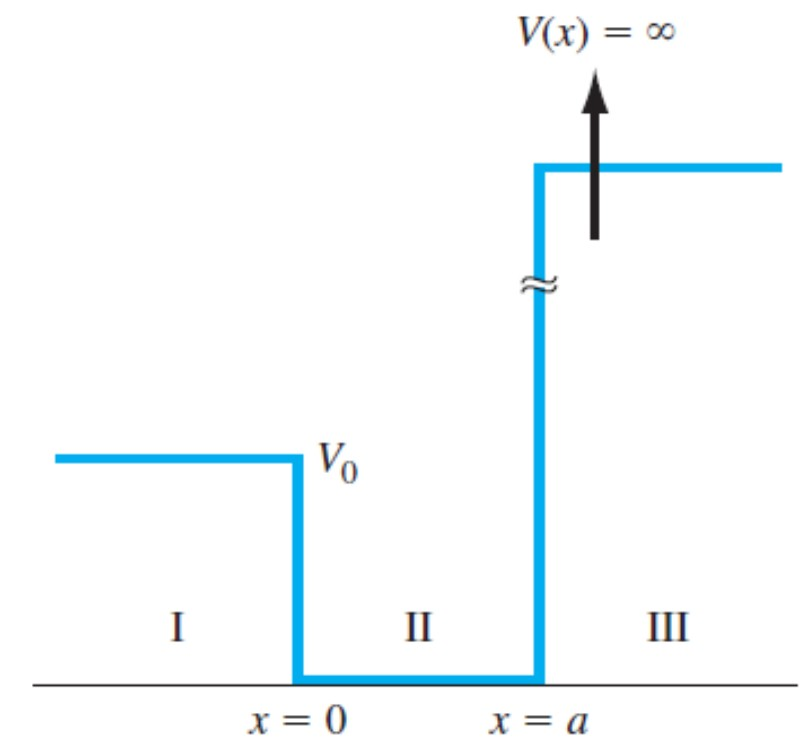
\includegraphics[width=0.4\linewidth]{Example-quantum-well.jpg}
            \label{fig:Example-quantum-well-2.jpg}
        \end{figure}
        \begin{equation*}
            \Psi(x) = \left\{
                \begin{array}{ll}
                    A \e^{-ik_1x} + B\e^{ik_1x} , & x \le 0\\
                    C \e^{-ik_2x} + D \e^{ik_2x}, & 0 < x < a \\
                    0, & x \ge a 
                \end{array}
            \right.
        \end{equation*}
        \begin{equation*}
            \left\{
                \begin{array}{ll}
                    & \Psi (x) | _{x = 0} \text{ continuous}\\
                    & \Psi (x) | _{x = a} \text{ continuous}\\
                    & \int_{-\infty}^{\infty} \Psi(x) \Psi^*(x) \d x = 1 \\
                \end{array}
            \right.
        \end{equation*}
    \end{frame}

    % * Chapter 3
\section{Chapter 3: Introduction to the Quantum Theory of Solids}
    \begin{frame} \frametitle{Energy bands}
        \begin{figure}[H]
            \centering
            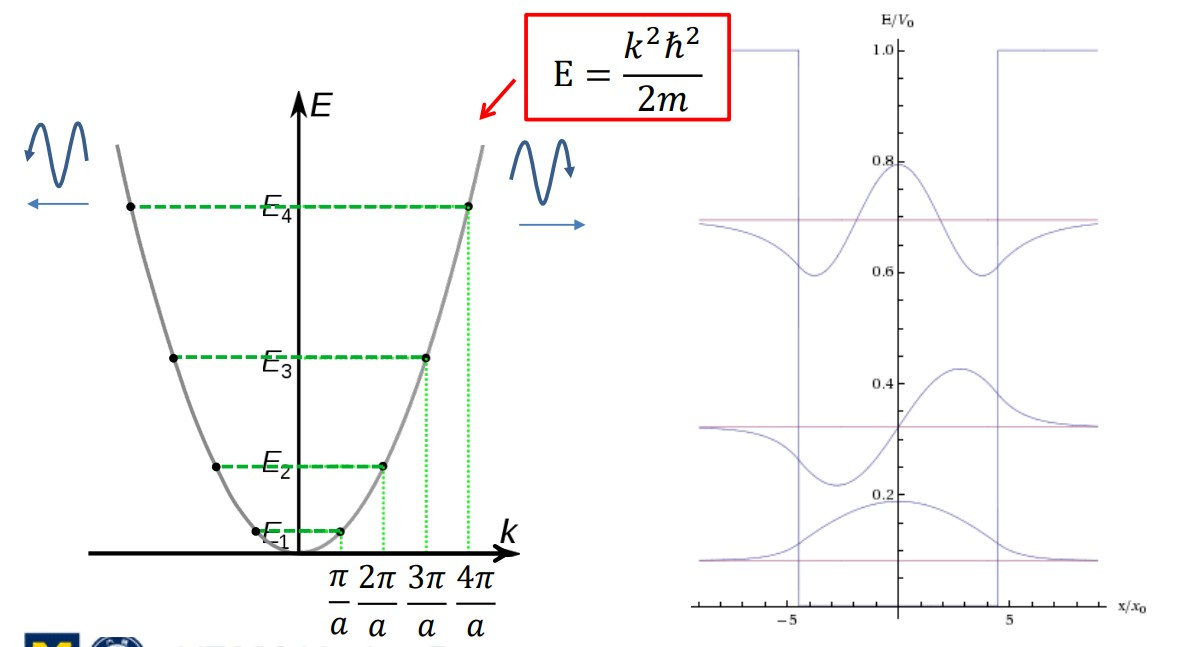
\includegraphics[width=0.6\linewidth]{Energy_bands.jpg}
            \label{fig:Energy_bands.jpg}
        \end{figure}
        \par For same energy level, the $k$ can have two values, Because the wave can move to positive and negative directions.
    \end{frame}

    \begin{frame} \frametitle{Effective mass}
        \begin{equation*}
            E = \frac{p^2}{2m} = \frac{k^2 \hbar^2}{2m} 
        \end{equation*}
        Taking derivative:
        \begin{equation*}
            \begin{aligned}
                & \frac{\d E}{\d k} = \frac{\hbar^2 k}{m} \\
                & \frac{1}{\hbar^2} \frac{\mathrm{d}^2 E}{\mathrm{d} k^2} = \frac{1}{m} 
            \end{aligned}
        \end{equation*}

        \begin{figure}[H]
            \vspace{-0.5em}
            \centering
            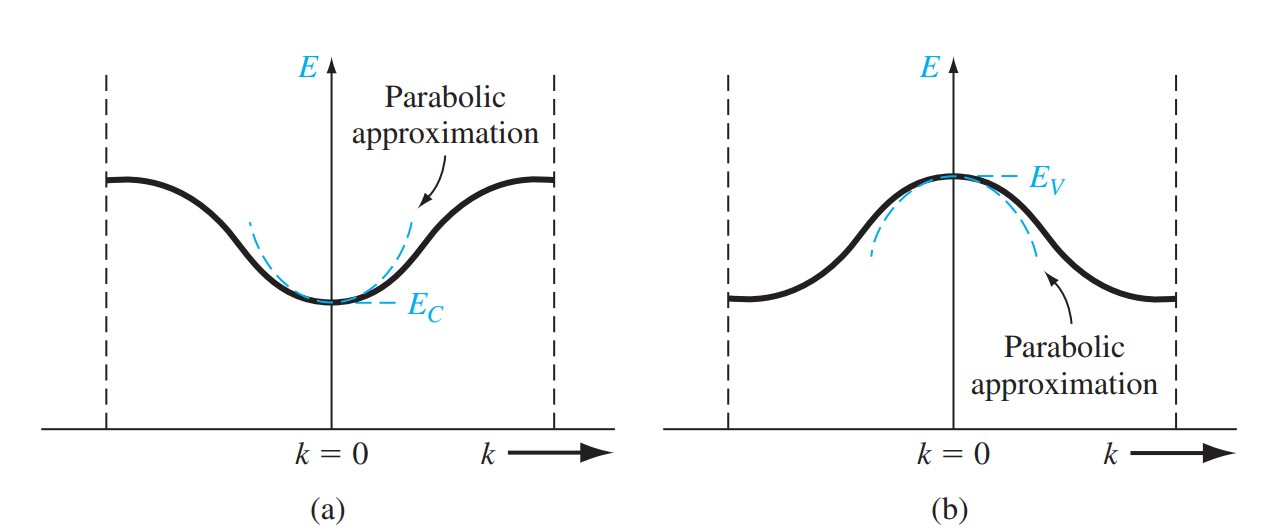
\includegraphics[width=0.7\linewidth]{Effective-mass.jpg}
            \caption{\tiny (a) The conduction band in reduced k space, and the parabolic approximation. (b) The valence band in reduced k space, and the parabolic approximation}
            \label{fig:Effective-mass.jpg}
            \vspace{-0.5em}
        \end{figure}
        \begin{equation*}
            E - E_c = C_1 k^2
        \end{equation*}
    \end{frame}

    \begin{frame} \frametitle{Effective mass}
        \begin{equation*}
            \boxed{\frac{1}{\hbar^2} \frac{\d^2 E}{\d k^2} = \frac{2C_1}{\hbar^2} = \frac{1}{m^*}  }
        \end{equation*}
        \begin{equation*}
            \begin{aligned}
                E = E(k) = E_c + \frac{\hbar^2}{2m_n^*} (k - k_1)^2 \\
                E = E(k) = E_v - \frac{\hbar^2}{2m_p^*} (k - k_2)^2
            \end{aligned}
        \end{equation*}
    \end{frame}

    \begin{frame} \frametitle{Example}
        A simplified $E$ versus $k$ curve for an electron in the conduction band is given. The value of $a$ is $10 \; \mathring{A}$. Determine the relative effective mass $m^* / m_0$.
        \begin{figure}[H]
            \centering
            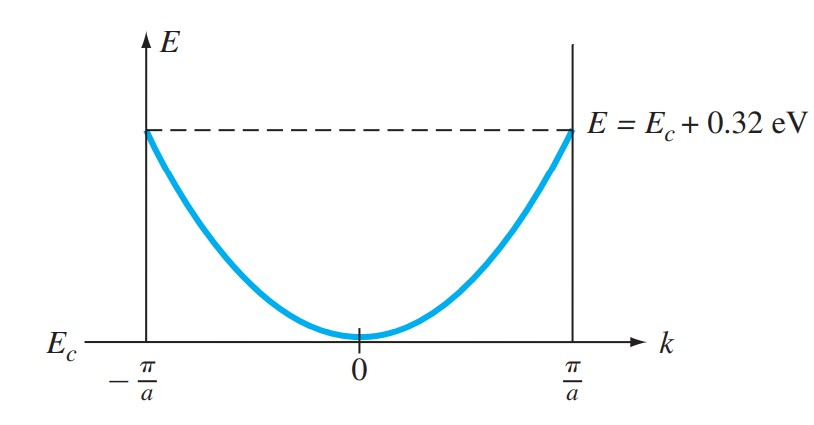
\includegraphics[width=0.6\linewidth]{Example-effective-mass.jpg}
            \label{fig:Example-effective-mass.jpg}
        \end{figure}
        Answer: \fbox{\textcolor{white}{1.175}}
    \end{frame}

    \begin{frame} 
        \begin{center}
            \Large\textcolor{blue}{End}
        \end{center}
    \end{frame}

\end{document}